\documentclass[11pt,a4paper]{article}
\usepackage[margin=25mm]{geometry}
\usepackage[T1]{fontenc}
\usepackage{lmodern}
\usepackage{xcolor}
\usepackage{booktabs}
\usepackage{hyperref}
\usepackage{tikz}
\usetikzlibrary{arrows.meta,positioning}

\definecolor{policy}{HTML}{7A3E9D}
\definecolor{kernel}{HTML}{176B87}
\definecolor{storage}{HTML}{2E7D32}
\hypersetup{colorlinks=true,linkcolor=policy,urlcolor=kernel}

\title{permfs: a Policy Layer over Linux OverlayFS}
\author{permfs}
\date{\today}

\begin{document}
\maketitle

\begin{abstract}
permfs is a library that presents a filesystem through a dynamic path
policy. Linux OverlayFS stores all changes. A low-level FUSE filesystem
controls namespace visibility and decides whether each path is read-only,
writable, or requires an interactive decision. This split keeps filesystem
mechanics in the kernel and keeps the policy implementation small.
\end{abstract}

\section{Stack}

\begin{center}
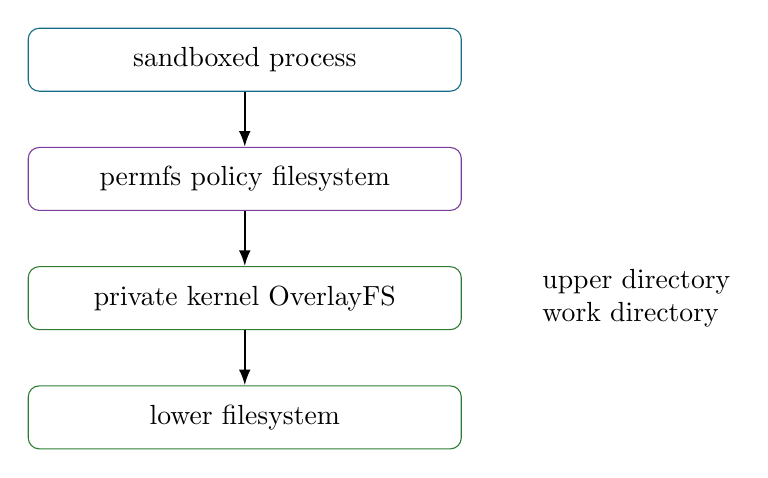
\begin{tikzpicture}[
  node distance=7mm,
  box/.style={draw,rounded corners,minimum width=55mm,minimum height=8mm},
  arrow/.style={-{Latex[length=2mm]},thick}
]
\node[box,draw=storage] (lower) {lower filesystem};
\node[box,draw=storage,above=of lower] (overlay) {private kernel OverlayFS};
\node[box,draw=policy,above=of overlay] (fuse) {permfs policy filesystem};
\node[box,draw=kernel,above=of fuse] (task) {sandboxed process};
\draw[arrow] (task) -- (fuse);
\draw[arrow] (fuse) -- (overlay);
\draw[arrow] (overlay) -- (lower);
\node[right=9mm of overlay,align=left] {upper directory\\work directory};
\end{tikzpicture}
\end{center}

OverlayFS performs copy-up, whiteouts, opaque directory handling, sparse file
I/O, mmap, hard links, and rename. The FUSE layer does not reproduce those
operations. It checks policy and forwards permitted calls to the merged mount.

\section{Policy}

Rules are stored in a memory-mapped radix trie. Lookup returns the nearest
explicit slash-component ancestor.

\begin{center}
\begin{tabular}{ll}
\toprule
Rule & Result\\
\midrule
\texttt{whiteout} & the path appears not to exist\\
\texttt{r} & metadata and read-only opens\\
\texttt{rw} & reads and mutations may continue\\
\texttt{ask} & obtain and store a decision before continuing\\
\bottomrule
\end{tabular}
\end{center}

The zero trie value is reserved for an internal node without an explicit
rule. Durable rules therefore use nonzero values.

An ask operation checks the trie a second time before prompting. Prompt locks
are striped by path hash, so two requests for one path do not create duplicate
questions while unrelated paths can continue independently. The returned
decision is written as an explicit rule before the original operation opens a
handle.

\section{Unix permissions}

The FUSE mount uses \texttt{default\_permissions} and returns ownership and
mode metadata from the merged OverlayFS object. The kernel checks the caller's
UID, GID, mode bits, ACL, sticky directory rules, and execute permission.
permfs then applies its four-state path policy. OverlayFS finally performs
the operation using its mount credentials.

This arrangement avoids a partial userspace implementation of supplementary
groups, ACLs, capabilities, and sticky directories.

\section{Open handles and passthrough}

Policy is resolved before opening a handle. A handle stores one access byte.
Read, write, flush, fsync, and release do not lock or read the trie. Later
policy changes affect later operations and opens, not an existing resolved
descriptor.

When supported, the daemon registers the merged OverlayFS descriptor with
FUSE passthrough. Kernel read, write, splice, and mmap can then use that
descriptor directly. A read-only rule receives a read-only descriptor. A
writable rule receives the flags requested by the caller. The normal FUSE I/O
path is used when passthrough is unavailable.

\section{Concurrency}

The inode map lock covers only publication and reference counts. No backing
filesystem syscall runs while that lock is held. An inode is destroyed only
after its FUSE lookup count and open-handle count both reach zero. This makes
concurrent forget and release operations safe.

The policy trie uses a \texttt{std.Io.RwLock}. Individual lookups hold its read
side. Rule batches and ask decisions hold its write side for their complete
transaction.

\section{Session layout}

A session directory contains:

\begin{verbatim}
session/
  lock
  upper/
  work/
  merged/
\end{verbatim}

The lock prevents two drivers from mounting or applying one session. Upper
and work are on the same filesystem. The initial mount requests
\texttt{redirect\_dir=on}, \texttt{index=on}, \texttt{xino=auto}, and
\texttt{metacopy=off}. If inode indexing is unsupported, the mount retries
without it and logs the result.

\section{Apply and recovery}

Apply is allowed only after both mounts have stopped. It walks the upper tree.
Regular files are copied into a destination-side temporary file. The temporary
file is synced and renamed over its destination. The destination directory is
then synced. Only after those steps does apply remove the upper entry.

Whiteouts delete the corresponding lower object. Opaque directories replace
the lower directory contents. Symlinks and special files are recreated.
OverlayFS bookkeeping attributes are not copied into the lower tree.

The upper tree is the checkpoint. A crash before upper removal repeats an
idempotent publication. A crash after upper removal has already completed
that operation. A bounded apply leaves remaining upper entries for the next
call. Discard removes one selected upper subtree.

\section{Limits}

Editing an OverlayFS lower tree while it is mounted is unsupported by Linux.
permfs does not attempt to make it safe. Kernel OverlayFS and FUSE support,
mount privileges, upper filesystem xattrs, and valid directory entry types
are required. Passthrough additionally needs kernel support and
\texttt{CAP\_SYS\_ADMIN}.

\end{document}
